\documentclass[twoside]{amsart}
\usepackage{amssymb,latexsym}
\usepackage{amsfonts}
\usepackage{xspace}
\usepackage{enumerate}
\usepackage{graphics}
\usepackage{fitch}
\newcommand{\Rationals}{\mathbb{Q}{}}
\newcommand{\Reals}{\mathbb{R}{}}
\newcommand{\Integers}{\mathbb{Z}{}}
\newcommand{\solution}{\textsc{Solution}\xspace}
\newcommand{\problem}{\textsc{Problem}\xspace}
\newcommand{\Blank}{\mathrel{\phantom{=}}}
\newcommand{\ltrue}{\top}
\newcommand{\lfalse}{\bot}
\begin{document}
\title{Answers to Chapter 5 Exercises - A Book of Abstract Algebra}
\author{Michael Welch}
\date{\today}
\maketitle

This document contains selected answers to exercises from chapter 5
of A Book of Abstract Algebra.


\begin{enumerate}[A.]
   \item \textsc{Recognizing Subgroups}

   \noindent In parts 1--6 below, determine whether or not $H$ is a
   subgroup of $G$. (Assume that the operation of $H$ is the same as
   that of $G$.)

   \textbf{Instructions} If $H$ is a subgroup of $G$, show that
   both conditions in the definition of ``subgroup'' are satisfied.
   If $H$ \emph{is not} a subgroup of $G$, explain which condition
   fails.
  

   \noindent 1. $G = \langle \mathbb{R},+ \rangle,\, H = 
   \{\log a : a \in \mathbb{Q}, a > 0 \}$.

   \noindent \solution $H$ is a subgroup of $G$:
   \begin{enumerate}[(i)]
      \item Assume $\log a, \log b \in H$. Since $a,b$ are rational numbers
      there are numbers $m_1,n_1,m_2,n_2$ such that $a = m_1/n_1, b = m_2/n_2$.
      So we have 
      \begin{align*}
         \log a + \log b & = \log \frac{m_1}{n_1} + \log \frac{m_2}{n_2} \\
	                 & = \log m_1 - \log n_1 + \log m_2 - \log n_2 \\
			 & = \log m_1m_2 - \log n_1n_2 \\
			 & = \log \frac{m_1m_2}{n_1n_2}
      \end{align*}

      Since $\displaystyle \frac{m_1m_2}{n_1n_2} \in \mathbb{Q}$ 
      we have that $H$ is closed with respect to addition.

      \item Assume $\log a \in H$. Again we know that there are numbers
      $m,n$ such that $a = m/n$. So we have
      \begin{align*}
         - \log a & = - \log \frac{m}{n} \\
	          & = - (\log m - \log n) \\
		  & = \log n - \log m \\
		  & = \log \frac{n}{m}
      \end{align*}

      Since $\displaystyle \frac{n}{m} \in \mathbb{Q}$ we have that 
      $H$ is closed with respect to inverses.
   \end{enumerate}

   \noindent 2. $G = \langle \mathbb{R}, + \rangle,\, H = 
   \{ \log n : n \in \mathbb{Z}, n > 0\}$.

   \noindent \solution It is rather easy to show that $H$ is closed
   with respect to addition (following a procedure similar to the
   previous example). However, it is not closed with respect to
   inverses:
      \begin{align*}
         - \log n & = - \log \frac{n}{1} \\
	          & = - (\log n - \log 1) \\
		  & = \log 1 - \log n \\
		  & = \log \frac{1}{n}
      \end{align*}

   Since $\displaystyle \frac{1}{n} \not \in \mathbb{Z}$, $H$ is
   not closed with respect to inverses.

   \noindent 3. $G = \langle \mathbb{R},+ \rangle,\, H = 
   \{ x \in \mathbb{R} : \tan x \in \mathbb{Q}\}$. \textsc{Hint}:
   Use the following formula from trigonometry:
   \[
      \tan (x+y) = \frac {\tan x + \tan y}{1 - \tan x \tan y}
   \]

   \noindent \solution Assume $x,y \in \mathbb{R}$ and $\tan x,
   \tan y \in \mathbb{Q}$. We know that $x+y \in \mathbb{R}$.
   We need to check that $\tan (x+y) \in \mathbb{Q}$. Choose 
   $m_1,n_1,m_2,n_2 \in \mathbb{Z}$ such that $\tan x = m_1/n_1$
   and $\tan y = m_2/n_2$.
   \begin{align*}
      \tan (x + y) & = \frac {\tan x + \tan y}{1 - \tan x \tan y}\\
                   & = \frac {m_1/n_1 + m_2/n_2}{1 - m_1m_2/n_1n_2} \\
   \end{align*}

   This shows us that $H$ is not closed with respect to addition. If
   $\tan x \tan y = 1$ then we have $\displaystyle \tan (x+y) =
   \frac{\tan x + \tan y}{0} \not \in \mathbb{Q}$.

   \noindent 4. $G = \langle \mathbb{R}^*,\cdot \rangle,\, H =
   \{2^n3^m : m,n \in \mathbb{Z}\}$.   
   
   \noindent \solution 
   \begin{enumerate}[(i)]
      \item Assume that we have two numbers $2^{n_1}3^{m_1}, 2^{n_2}3^{m_2} \in
      H$.  $2^{n_1}3^{m_1}\cdot 2^{n_2}3^{m_2} = 2^{n_1+n_2}3^{m_1+m_2}$, and
      $n_1+n_2,m_1+m_2 \in \mathbb{Z}$. So $H$ is closed with respect to
      multiplication.

      \item Assume that we have a number $2^n3^m \in H$. Then
      $1/2^n3^m = 2^{-n}3^{-m}$, and $-n, -m \in \mathbb{Z}$. So
      $H$ is closed with respect to multiplicative inverses.
   \end{enumerate}

   \noindent 5. $G = \langle \mathbb{R} \times \mathbb{R},+ \rangle,\, H =
   \{ (x,y) : y = 2x\}$.

   \noindent \solution 
   
   \begin{enumerate}[(i)]
      \item Assume we have two tuples $(x_1,y_1),(x_2,y_2) \in H$. Then
      $(x_1,y_1)+(x_2,y_2) = (x_1+x_2,y_1+y_2)$. Since we know that $y_1 =
      2x_1$ and $y_2 = 2x_2$ we have $y_1+y_2 = 2x_1 + 2x_2 = 2(x_1+x_2)$.
      Therefore, $H$ is closed with respect to addition.

      \item Assume we have a tuple $(x,y)\in H$. The inverse is
      $(-x,-y)$. We know $y=2x$, so we have $-y = -2x = 2 \cdot -x$.
      Therefore, $H$ is closed with respect to inverses.

   \end{enumerate}

   \noindent 6. $ G =\langle \mathbb{R} \times \mathbb{R}, + \rangle,\, H=
   \{(x,y) : x^2 + y^2 > 0\}$.

   \noindent \solution 
   \begin{enumerate}[(i)]
      \item Assume we have two tuples $(x_1,y_1),(x_2,y_2)\in H$. Then
      $(x_1,y_1) + (x_2,y_2) = (x_1+x_2,y_1+y_2)$. $(x_1+x_2)^2 +
      (y_1+y_2)^2 = x_1^2 + 2x_1x_2 + x_2^2 + y_1^2 + 2y_1y_2 + y_2^2$.
      We can find values of $x_1,x_2,y_1,y_2$ such that 
      $ x_1^2 + 2x_1x_2 + x_2^2 + y_1^2 + 2y_1y_2 + y_2^2 = 0$. For example,
      choose the tuples $(-\frac{1}{4},\frac{1}{4})$ and $(\frac{1}{4},
      - \frac{1}{4})$. When we add them together we get $(0,0)$. 
      $0^2 + 0^2 \not > 0$.
      Therefore, $H$ is not closed with respect to addition.
   \end{enumerate}

   \noindent 7. Let $C$ and $D$ be sets, with $C \subseteq D$. Prove
   that $P_C$ is a subgroup of $P_D$. (See Chapter 3, Exercise C.)
   As a reminder the operation on $P_D$ is the \emph{symmetric difference},
   $\ominus$.

   \noindent \solution  $\langle P_C,\ominus \rangle$ is a subgroup of
   $\langle P_D,\ominus \rangle$.
   
   \begin{enumerate}[(i)]
      \item Assume we have two sets $A,B \in P_C$. We know $P_C = \{ A' : A'
      \subseteq C\}$. Therefore, $A \subseteq C$ and $B \subseteq C$. If we
      remove any elements from $A$ or $B$ it is obvious the result is also a
      subset of $C$. Next I need to mention that the union of any two subsets
      of $C$ is also a subset of $C$.  We have $A \ominus B = (A - B) \cup (B -
      A)$. Since $A-B\subseteq C$ and $B-A\subseteq C$ and $(A-B)\cup (B-A)
      \subseteq C$ we have that $P_C$ is closed with respect to $\ominus$.


      \item From Chapter 3 Exercise C we know that the inverse of A is A. 
      Therefore $\langle P_C, \ominus \rangle$ is closed with respect
      to inverses. 
   \end{enumerate} 

   \item \textsc{Subgroups of Functions}

   \noindent In each of the following, show that $H$ is a subgroup of $G$.

   \noindent 1. \problem $G = \langle \mathcal{F}(\mathbb{R}), + \rangle,\, H=
   \{ f \in \mathcal{F}(\mathbb{R}) : f(x) = 0 \text{ for every } 
   x \in [0,1]\}$.

   \noindent \solution We will show $H$ is a subgroup of $G$.
   
   \begin{enumerate}[(i)]
      \item Assume we have $f,g \in H$; then $f(x) = 0$ for $x \in [0,1]$ and
      $g(x) = 0$ for $x \in [0,1]$. So $[f+g](x) = f(x) + g(x) = 0 + 0 = 0$ for
      $x \in [0,1]$. Thus $f+g \in H$.

      \item If $f \in H$, then $f(x) = 0$ for $x \in [0,1]$. Thus,
      $[-f](x)=-f(x)=-0=0$ for $x \in [0,1]$. So $-f \in H$.

   \end{enumerate}

   \noindent 2. \problem $G = \langle \mathcal{F}(\mathbb{R}), + \rangle,\, H =
   \{ f \in \mathcal{F}(\mathbb{R}) : f(-x) = -f(x)\}$.

   \noindent \solution We will show $H$ is a subgroup of $G$.

   \begin{enumerate}[(i)]
      \item Suppose $f,g\in H$; then $f(-x) = -f(x)$ and $g(-x) = -g(x)$.
      So $[f+g](-x) = f(-x) + g(-x) = -f(x) - g(x) = -(f(x) + g(x)) = 
      - [f+g](x)$. Thus, $f+g\in H$.

      \item Suppose $f \in H$; then $f(-x)= -f(x)$. Thus 
      $[-f](-x) = -f(-x) = -(-f(x)) = f(x)$. Thus, $f\in H$.
   \end{enumerate}

   \noindent 3. \problem  $G=\langle \mathcal{F}(\mathbb{R}),+\rangle,\, H=
   \{ f \in \mathcal{F}(\mathbb{R}) : f \text{ is periodic of period $\pi$}\}$

   \noindent \textsc{Remark:} A function $f$ is said to be \emph{periodic}
   of period $a$ if there is a number $a$, called the period of $f$,
   such that $f(x) = f(x+na)$ for every $x \in \mathbb{R}$ and 
   $n \in \mathbb{Z}$.

   \noindent \solution 
   
   \begin{enumerate}[(i)]
      \item  Suppose $f,g \in H$; then $f(x) = f(x+na)$ and 
      $g(x) = g(x+na)$ for every $x \in \mathbb{R}$ and $n \in \mathbb{Z}$.
      So $[f+g](x) = f(x) + g(x) = f(x + na) + g(x+na)$ which equals
      $[f+g](x + na)$ for all $x\in \mathbb{R}$ and $n \in \mathbb{Z}$. 
      Thus, $f+g \in H$.
   \end{enumerate}

   \noindent 4. \problem $G = \langle \mathcal{F}(\mathbb{R}),+\rangle,\, H=
   \{ f \in \mathcal{F}(\mathbb{R}) : \int_0^1 f(x) dx = 0\}$

   \noindent \solution 
   \begin{enumerate}[(i)]
      \item Suppose $f,g \in H$; then $\int_0^1 f(x) dx = 0$ and
      $\int_0^1 g(x)dx = 0$. So $[f+g](x) = f(x) + g(x)$ and
      $\int_0^1 (f(x)+g(x)) dx = \int_0^1 f(x)dx + \int_0^1 g(x)dx = 0$.
      Thus, $f+g \in H$.

      \item Suppose $f \in H$; then $[-f](x) = -f(x)$ and
      $\int_0^1 -f(x)dx = -\int_0^1 f(x) dx = -0 = 0$. Thus, $-f \in H$.
   \end{enumerate}

   \noindent 5. \problem $G = \langle \mathcal{F}(\mathbb{R}),+\rangle,\, H =
   \{ f \in \mathcal{F}(\mathbb{R}) : df/dx \text{ is constant}\}$

   \noindent \solution 
   \begin{enumerate}[(i)]
      \item Suppose $f,g \in H$; then $[f+g](x) = f(x) + g(x)$, and
      $df/dx = k_1$ and $dg/dx = k_2$ and 
      $d(f+g)/dx = df/dx + dg/dx = k_1 + k_2 = k_3$. So $k_3$ is a constant
      and $f+g\in H$.

      \item Suppose $f \in H$; then $[-f](x) = -f(x)$, and
      $d(-f)/dx = -df/dx = -k$. Thus, $-f \in H$.
   \end{enumerate}

   \noindent 6. \problem $G=\langle \mathcal{F}(\mathbb{R}),+\rangle,\, H =
   \{ f \in \mathcal{F}(\mathbb{R}) : f(x) \in \mathbb{Z}$ for every
   $x \in \mathbb{R}\}$.

   \noindent \solution 
   \begin{enumerate}[(i)]
      \item Suppose $f,g \in H$; then $f(x)\in\mathbb{Z}$ and
      $g(x)\in\mathbb{Z}$ for every $x\in\mathbb{R}$. So
      $[f+g](x)=f(x)+g(x)$ and $f(x)+g(x) \in \mathbb{Z}$ for every
      $x \in \mathbb{R}$.

      \item Suppose $f \in H$; then $[-f](x)=-f(x)$. But $-f(x) \in 
      \mathbb{Z}$ for every $x \in \mathbb{R}$.
   \end{enumerate}

   \item \textsc{Subgroups of Abelian Groups}

   \noindent In the following exercises, let $G$ be an abelian group.

   \noindent 1. If $H=\{x \in G : x = x^{-1}\}$, that is, $H$ consists of
   all the elements of $G$ which are their own inverses, prove that $H$
   is a subgroup of $G$.

   \noindent \solution Suppose $x,y \in H$; then $x=x^{-1}$ and $y=y^{-1}$.
   So $xy = x^{-1}y^{-1} = (yx)^{-1} = (xy)^{-1}$. Thus $xy \in H$; and
   by definition $x^{-1} \in H$.

   \noindent 2. Let $n$ be a fixed integer, and let $H=\{x \in G
   : x^n = e\}$. Prove that $H$ is a subgroup of $G$.

   \noindent \solution 
   \begin{enumerate}[(i)]
      \item Suppose $x,y\in H$ then $x^n=e$ and $y^n=e$ and
	 \begin{align*}
	 (xy)^n & = \underbrace{(xy)(xy)(xy)\cdots (xy)}_{n \text{ factors}}\\
	        & = \underbrace{xxx\cdots x}_{n\text{ factors}}
		    \underbrace{yyy\cdots y}_{n\text{ factors}}
		    && \text{Commutative property} \\
		& = e
	 \end{align*}
      \item Supose $x\in H$ then $x^n = e$. Let's check if the inverse is
      in $H$.  
      \begin{align*}
          e & = x^n \\
	  e & = \underbrace{xx\cdots x}_{n\text{ factors}} \\
	  x^{-1} & = \underbrace{xx\cdots x}_{n-1\text{ factors}}\\
	  \underbrace{x^{-1}x^{-1}\cdots x^{-1}}_{n\text{ factors}} & = e \\
	  (x^n)^{-1} & = e
      \end{align*}

      Therefore $(x^n)^{-1} \in H$.
   \end{enumerate}

   \noindent 3. Let $H=\{x\in G : x = y^2 \text{ for some } y \in G\}$;
   that is, let $H$ be the set of all the elements of $G$ which
   have a square root. Prove that $H$ is a subgroup of $G$.

   \noindent \solution
   \begin{enumerate}[(i)]
      \item Suppose $a,b \in H$ then there are two elements $x,y\in G$
      such that $a=x^2, b=y^2$. 
      \begin{align*}
         ab & = x^2y^2 \\
	    & = xxyy   \\
	    & = xyxy   && \text{By commutativity} \\
	    & = (xy)^2
      \end{align*}
      Therefore, $ab$ has a square root and $ab \in H$.

      \item Suppose $x \in H$. Then $x=y^2$ for some $y \in G$. 
      \begin{align*}
         x & = y^2 \\
	 x^{-1} & = (y^2)^{-1} \\
	        & = (yy)^{-1} \\
		& = y^{-1}y^{-1} \\
		& = (y^{-1})^2
      \end{align*}
      Therefore $x^{-1}$ has an inverse and since $y^{-1}\in G$ 
      we have $x^{-1} \in H$.
   \end{enumerate}

   \noindent 4. Let $H$ be a subgroup of $G$, and let 
   $K = \{x \in G : x^2 \in H\}$. Prove that $K$ is a subgroup of $G$.

   \noindent \solution 
   \begin{enumerate}[(i)]
      \item Suppose $x,y \in K$. Therefore $x,y\in G$, and $x^2,y^2 \in H$.
      Since $G$ is group we know $xy \in G$. Since $H$ is a group we
      have that $x^2y^2 \in H$. But $x^2y^2 = xxyy = (xy)^2$ (by commutativity).
      Since $xy\in G$ and $(xy)^2 \in H$ we have that $xy \in K$ (by
      the definition of $K$.

      \item Suppose $x \in K$. Therefore $x \in G, x^2 \in H$. Since
      $G$ and $H$ are groups we have that $x^{-1} \in G$ and 
      $(x^2)^{-1} \in H$. But $(x^2)^{-1} = x^{-1}x^{1} = (x^{-1})^2$.
      Since $x^{-1} \in G$ and $(x^{-1})^2 \in H$, we have
      $x^{-1} \in K$.
   \end{enumerate}
   

   \noindent 5. Let $H$ be a subgroup of $G$, and let $K$ consist of all
   the elements $x$ in $G$ such that some power of $x$ is in $H$.
   That is, $K = \{x \in G : \text{ for some integer } n > 0,\,
   x^n \in H \}$. Prove that $K$ is a subgroup of $G$.

   \noindent \solution 
   \begin{enumerate}[(i)]
      \item Suppose $x,y \in K$. Then there are two numbers $m,n$ such that
      $x^m, y^n \in H$. Since H is a group it is closed to multiplication (and
      exponentiation). Therefore, $(x^m)^n, (y^n)^m \in H$. Set q = mn. Then
      $(xy)^q = (xy)^{mn} = x^{mn}y^{mn} = (x^m)^n(y^n)^m \in H$. Therefore $xy
      \in K$. (The step $(xy)^{mn}$ to $(x^{mn}y^{mn})$ relies on commutativty.)

      \item Suppose $x \in K$. Then we know $x^n \in H$ for some $n$. Since
      $H$ is a group $(x^n)^{-1} \in H$. Therfore, $(x^{-1})^n \in H$.
      Therefore $x^{-1} \in K$.
   \end{enumerate}

   \noindent 6. Suppose $H$ and $K$ are subroupgs of $G$, and define 
   $HK$ as follows
   \[
      HK = \{ xy : x \in H \text{ and } y \in K \}
   \]
   Prove that $HK$ is a subgroup of $G$.

   \noindent \solution
   \begin{enumerate}[(i)]
      \item Suppose $a,b \in HK$. Then there are elements $x_1,x_2 \in H$
      and $y_1,y_2 \in K$ such that $a=x_1y_1$ and $b=x_2y_2$.
      Therefore, $ab = x_1y_1x_2y_2$ which equals $(x_1x_2)(y_1y_2)$
      by commutativity. Since $H$ and $G$ are groups 
      $x_1x_2 \in H$ and $y_1y_2 \in G$. Therefore $x_1x_2y_1y_2 \in HK$.

      \item Suppose $xy \in HK$. Therefore $x,x^{-1} \in H$ and
      $y,y^{-1} \in G$. Therefore $x^{-1}y^{-1} in HK$. 
      But $x^{-1}y^{-1} = (yx)^{-1} = (xy)^{-1} \in HK$.
   \end{enumerate}

   \noindent 7. Explain why parts 4--6 are not true if $G$ is not abelian.
   \noindent \solution Each of the proof relied on re-ordering factors
   (using commutativity) to prove an identity. Without those steps
   the proof cannot be made.

   \item \textsc{Subgroups of an Arbitrary Group}

   \noindent Let $G$ be a group.

   \noindent 1. If $H$ and $K$ are subgroups of a group $G$, 
   prove that $H \cap K$ is a subgroup of $G$. (Remember, that
   $x\in H\cap K \text{ iff } x \in H \text{ and } x \in K$.)

   \noindent \solution 
   \begin{enumerate}[(i)]
      \item Suppose $x,y \in H \cap K$. Therefore, $x,y \in H$ and
      $x,y\in K$. Since $H$ and $K$ are both groups we know
      $xy \in H$ and $xy \in K$. So $xy \in H \cap K$.

      \item Suppose $x \in H \cap K$. Therefore $x$ is in both $H,K$. 
      Therefore $x^{-1}$ is in both $H,K$; and so $x^{-1} \in H \cap K$.
   \end{enumerate}

   \noindent 2. Let $H$ and $K$ be subgroups of $G$. Prove that
   if $H \subseteq K$, then $H$ is a subgroup of $K$.

   \noindent \solution Um, this seems like its true by definition.
   We know that $H$ is a group and that it's a subset of $K$.
   Therefore $H$ is a subgroup of $K$. Right? I mean $H$ is
   closed with respect to it's operation since it's a group. And
   it's closed with respect to inverses since it's a group. And
   it's a subset of $K$. That's the definition in paragraph 1 of
   this chapter.

   \noindent 3. By the \emph{center} of a group $G$ we mean the set of
   all the elements of $G$ which commute with every element of $G$,
   that is,
   \[
       C = \{ a\in G : ax = xa \text{ for every } x \in G\}
   \]
   Prove that $C$ is a subgroup of $G$.
   
   \noindent \solution 
   \begin{enumerate}[(i)]
      \item Suppose $a,b \in C$. This means $ax=xa$ and $bx=xb$ for every $x
      \in G$.  Choose any $x\in G$:
      \begin{align*}
         abx & = axb && \text{Given $bx=xb$} \\
	     & = xab && \text{Given $ax=xa$} 
      \end{align*}
      So $ab \in C$.

      \item Suppose $a \in C$. This means $ax=xa$ for every $x\in G$.
      Choose any $x\in G$.
      \begin{align*}
         ax & = xa \\
	 axa^{-1} & = xaa^{-1} \\
	 axa^{-1} & = x \\
	 a^{-1}axa^{-1} & = a^{-1}x \\
	 xa^{-1} & = a^{-1}x
      \end{align*}
      Therefore $a^{-1} \in C$.
   \end{enumerate}

   \noindent 4. Let $C' = \{ a\in G : (ax)^2 = (xa)^2 
   \text{ for every } x \in G\}$.  Prove that $C'$ is a subgroup of $G$.

   \noindent \solution
   \begin{enumerate}[(i)]
      \item Suppose $a,b \in C'$. Then $(ax)^2=(xa)^2$ and $(bx)^2=(xb)^2$
      for every $x \in G$. Choose any $x \in G$ and recall $ab \in G$.
      \begin{align*}
         (abx)^2 & = abxabx \\
	         & = axbaxb && \text{commutativity} \\
		 & = xabxab && \text{commutativity} \\
		 & = (xab)^2
      \end{align*}
      Therefore $ab \in C'$.

      \item Suppose $a \in C'$. Then $ax=xa$ for all $x \in G$.
      \begin{align*}
         (ax)^2 & = (xa)^2 \\
	 axax   & = xaxa \\
	 aaxx   & = xxaa \\
	 aaxxa^{-1}a^{-1} & = xx\\
	 xxa^{-1}a^{-1} & = a^{-1}a^{-1}xx \\
	 xa^{-1}xa^{-1} & = a^{-1}xa^{-1}x \\
	 (xa^{-1})^2    & = (a^{-1}x)^2
      \end{align*}
      Therefore $a^{-1} \in C'$.
   \end{enumerate}

   \noindent 5. Let $G$ be a \emph{finite} group, and let S be a nonempty 
   subset of $G$. Suppose $S$ is closed with respect to 
   multiplication. Prove that $S$ is a subgroup of $G$. (\textsc{Hint:} It
   remains to prove that $S$ contains $e$ and is closed with respect
   to inverses. Let $S=\{a_1,\ldots,a_n\}$. If $a_i \in S$, consider
   the \emph{distinct} elements $a_ia_1,a_ia_2,\ldots,a_ia_n$.)

   \noindent \solution
   \begin{proof}
   Suppose $S=\{a_1,\ldots,a_n\}$. And choose some $a_i \in S$. Consider
   the elements $a_ia_1,a_ia_2,\ldots,a_ia_n$. Assume those elements
   are not distinct. Then there is some $m,n$ such that $a_ia_m=a_ia_n$ 
   which implies $a_m=a_n$. But we assumed the original elements were
   all distinct. Therefore the elements $a_ia_1,a_ia_2,\ldots,a_ia_n$
   must all be distinct. Let's call that set $S'$.
   Since the size of $S$ and size of $S'$ are the same then one of the
   elements $a_m$ must have mapped $a_ia_m$ to $a_i$, and therefore
   $a_m=e$. Since there is a neutral element, and again since both sets are
   the same size there must be an inverse for each element.
   \end{proof}

   \noindent 6. Let $G$ be a group and $f : G \rightarrow G$ a function.
   A \emph{period} of $f$ is any element $a$ in $G$
   such that $f(x) = f(ax)$ for every $x \in G$. Prove: The set of
   all the periods of $f$ is a subgroup of $G$.

   \noindent \solution 
   \begin{enumerate}[(i)]
      \item Suppose $a,b$ are periods of $f$. Then $f(x)=f(ax)$ and
      $f(x)=f(bx)$ for all elements $x\in G$. The elements $bx \in G$
      for all values of $x \in G$. Therefore $f(bx) = f(abx)$ for
      all $x \in G$. So we have $f(x)=f(abx)$ for all $x \in G$.
      Therefore $ab$ is a period of $f$.

      \item Suppose $a$ is a period of $f$. Then $f(x)=f(ax)$ for
      all $x$ in $G$. Now choose $y=a^{-1}x$ for some $x$. Then we have
      $y \in G$ so $f(ay) = f(y)$ for all values of $y$. So we have
      $f(ay) = f(y)$ or $f(aa^{-1}x) = f(a^{-1}x)$. But $f(aa^{-1}x) =
      f(x)$. So $f(a^{-1}x) = f(x)$. Therefore $a^{-1}$ is a period
      of $f$.

   \end{enumerate}

   \noindent 7. Let $H$ be a subgroup of $G$, and let $K = \{
      x \in G : xax^{-1} \in H \text{ iff } a \in H \}$. Prove:
      \begin{enumerate}[(a)]
         \item $K$ is a subgroup of $G$.
	 \item $H$ is a subgroup of $K$.
      \end{enumerate}

      The first proof for (a).

\begin{equation*}
   \begin{fitch}
      \fa x(yay^{-1})x^{-1} \in H \to yay^{-1} \in H & Given\\
      \fj xya(xy)^{-1} \in H  & $\mathbf{A}$\\
      \fa xyay^{-1}x^{-1} \in H & 2 Theorem 2\\
      \fa xyay^{-1}x^{-1} \in H \to yay^{-1} \in H & 1 Associativity\\
      \fa yay^{-1} \in H                   & 3, 4 $\to \mathbf{E}$\\
      \fa yay^{-1} \in H \to a \in H       & Given \\
      \fa a \in H                          & 5, 6 $\to \mathbf{E}$\\
      xya(xy)^{-1} \in H \to a \in H  & 2-7 $\mathbf{I}$\\
   \end{fitch}
\end{equation*}


    \item \textsc{Generators of Groups}

    \noindent 1. List all the cyclic subgroups of $\langle\,
    \mathbb{Z}_{10}, + \rangle$.

    \noindent \solution. 
    \begin{itemize}
        \item $\langle \{0\}, +\rangle$
	\item $\langle \{0,1,2,3,4,5,6,7,8,9\}, +\rangle$
	\item $\langle \{0,2,4,6,8\}, +\rangle$
	\item $\langle \{0,5\}, +\rangle$
    \end{itemize}

    \noindent 2. Show that $\mathbb{Z}_{10}$ is generated by 2 and 5.

    \noindent \solution So we have the group $\langle \{0,1,2,3,4,5,
    6,7,8,9\}, +\rangle$. The suggested generators are 2 and 5. We need
    to list the defining equations:
    \begin{align*}
       2 + 2 + 2 + 2 + 2 &= 0 \\
           2 + 2 + 2 + 5 &= 1 \\
                       2 &= 2 \\
       2 + 2 + 2 + 2 + 5 &= 3 \\
                   2 + 2 &= 4 \\
                       5 &= 5 \\
               2 + 2 + 2 &= 6 \\
                   2 + 5 &= 7 \\
           2 + 2 + 2 + 2 &= 8 \\
               2 + 2 + 5 &= 9 
    \end{align*}

    \noindent 3. Describe the subgroup of $\mathbb{Z}_{12}$ generated by
    6 and 9.

    \noindent \solution We will list the items that we can generated:
    \begin{align*}
       6 + 6 &= 0 \\
       6 + 9 &= 3
    \end{align*}
    So the subgroup is $\langle \{0,3,6,9\}, + \rangle$.

    \noindent 4. Describe the subgroup of $\mathbb{Z}$ generated by 10 and 15.
    
    \noindent \solution The subgroup is $\langle \{\dots,-20,-15,-10,-5,0,5,
    10,15,20,25,30,\dots\}, + \rangle$. 

    \noindent 5. Show that $\mathbb{Z}$ is generated by 5 and 7.

    \noindent \solution It is enough to show that 1 and -1 can be generated.
    From there we know we can generate every element in $\mathbb{Z}$.
    We have $5+5+5+5-7-7-7=-1$ and $7+7+7-5-5-5-5=1$.

    \noindent 6. Show that $\mathbb{Z}_2 \times \mathbb{Z}_3$ is a cyclic
    group. Show that $\mathbb{Z}_3 \times \mathbb{Z}_4$ is a cyclic group.

    \noindent \solution We must identify the generator. I believe in both
    cases the generator is $(1,1)$. First for $\mathbb{Z}_2 \times
    \mathbb{Z}_3$.
    \begin{align*}
        (1,1) + (1,1) &= (0,2) \\
	(0,2) + (1,1) &= (1,0) \\
	(1,0) + (1,1) &= (0,1) \\
	(0,1) + (1,1) &= (1,2) \\
	(1,2) + (1,1) &= (0,0) \\
	(0,0) + (1,1) &= (1,1)
    \end{align*}

    Next for $\mathbb{Z}_3 \times \mathbb{Z}_4$:
    \begin{align*}
        (1,1) + (1,1) &= (2,2) \\
	(2,2) + (1,1) &= (0,3) \\
	(0,3) + (1,1) &= (1,0) \\
	(1,0) + (1,1) &= (2,1) \\
	(2,1) + (1,1) &= (0,2) \\
	(0,2) + (1,1) &= (1,3) \\
	(1,3) + (1,1) &= (2,0) \\
	(2,0) + (1,1) &= (0,1) \\
	(0,1) + (1,1) &= (1,2) \\
	(1,2) + (1,1) &= (2,3) \\
	(2,3) + (1,1) &= (0,0) \\
	(0,0) + (1,1) &= (1,1)
    \end{align*}

    \noindent 7. Show that $\mathbb{Z}_2 \times \mathbb{Z}_4$ is not a cyclic
    group but is generated by $(1,1)$ and $(1,2)$. 
    
    \noindent \solution Well we know that
    $(0,x)$ for any $x \in \mathbb{Z}_4$ is not a generator because it
    never generates a value $(1,y)$ for any $y \in \mathbb{Z}_4$. So we
    can try all 4 possible generator values: $(1,0)$, $(1,1)$, $(1,2)$,
    and $(1,3)$. The first, $(1,0)$, can be eliminated as well since
    0 is the neutral element of $\mathbb{Z}_4$. 

    The tuple $(1,1)$ generates these values: $(1,1), (0,2), (1,3), (0,0)$
    and back to 
    $(1,1)$. So it doesn't generate $(0,1), (0,3), (1,0), (1,2)$.

    The tuple $(1,2)$ generates these values: $(1,2), (0,0)$ and back to 
    $(1,2)$.

    The tuple $(1,3)$ generates these values $(1,3), (0,2), (1,1), (0,0)$
    and back to $(1,3)$. 

    Now we can demonstrate that it is generated by $(1,1)$ and $(1,2)$.
    Here are the defining equations.
    \begin{align*}
                        (1,2) + (1,2) &= (0,0) \\
        (1,1) + (1,1) + (1,1) + (1,2) &= (0,1) \\
                        (1,1) + (1,1) &= (0,2) \\
	                (1,1) + (1,2) &= (0,3) \\
	        (1,1) + (1,1) + (1,2) &= (1,0) \\
	                        (1,1) &= (1,1) \\
                                (1,2) &= (1,2) \\
                (1,1) + (1,1) + (1,1) &= (1,3) 
    \end{align*}

    \noindent 8. Suppose a group $G$ is generated by two elements
    $a$ and $b$. If $ab=ba$, prove that $G$ is abelian.
    
    \noindent \solution Proof sketch. Let $x$ and $y$ be elements
    in $G$. So we know they each contain any number of $a$,$b$,$a^{-1}$,
    and $b^{-1}$ elements combined in any order. We will assume
    that there are no cases where the inverses are next to each other
    since they cancel each other out. So at every position we could
    have an $a$ followed by
    an $a$, $b$ or $b^{-1}$ or nothing. 
    Likewise we could have a $b$ followed by an $a$, $a^{-1}$, $b$ or
    nothing. First let's show that $ab^{-1}=b^{-1}a$:

    \begin{align*}
              ab &= ba \\
	abb^{-1} &= bab^{-1} \\
	       a &= bab^{-1} \\
	 b^{-1}a &= b^{-1}bab^{1}\\
	 b^{-1}a &= ab^{-1}
    \end{align*}

    Using a similar derivation it can be shown that $a^{-1}b = ba^{-1}$. 
    So using these commutativity facts we can start rearranging the order
    of elements in the combined term $xy$ so that all the $a$ elements
    come first and all of the $b$ elements come second. Anytime two
    inverses come into contact we'll cancel them out. This means
    we'll always end up with a sequence of 0 or more $a$ elements
    followed by 0 or more $b$ elements or just $e$. The same result
    will be obtained if we start with the combined term $yx$. (Actually
    it could be that the inverses of $a$ outnumber the $a$ elements
    and we have 1 or more $a^{-1}$ elements on the left. Likewise
    with $b^{-1}$ on the right.)

    \item \textsc{Groups Determined by Generators and Defining Equations}

    \noindent 1. Let $G$ be the group $\{e,a,b,b^2,ab,ab^2\}$ whose 
    generators satisfy $a^2 = e$, $b^3 = e$, and $ba = ab^2$.
    Write the table of $G$.

    \begin{center}
    \begin{tabular}{c|cccccc}
%   12345678 12345678 12345678 12345678 12345678 12345678 12345678
    $\cdot$ & $e$    & $a$    & $b$    & $b^2$  & $ab$   & $ab^2$ \\ \hline
     $e$    & $e$    & $a$    & $b$    & $b^2$  & $ab$   & $ab^2$ \\
     $a$    & $a$    & $e$    & $ab$   & $ab^2$ & $b$    & $b^2$  \\
     $b$    & $b$    & $ab^2$ & $b^2$  & $e$    & $a$    & $ab$   \\

% (bb)a = babb = abbbb = ab
% (bb)ab = b(ba)b = b(abb)b = (ba) = abb
% (bb)abb = b(ba)bb = b(abb)bb = bab = abbb = a
     $b^2$  & $b^2$  & $ab$   & $e$    & $b$    & $ab^2$ & $a$    \\

% (ab)a = a(ba) = a(abb) = (aa)(bb) = bb
% (ab)(ab) = a(ba)b = a(abb)b = (aa)(bbb) = e
     $ab$   & $ab$   & $b^2$  & $ab^2$ & $a$    & $e$    & $b$    \\

% (abb)a = (ab)(ba) = (ab)(abb) = a(ba)bb = a(abb)bb = (aa)(bbb)b = b
% (abb)ab = bb
     $ab^2$ & $ab^2$ & $b$    & $a$    & $ab$   & $b^2$  & $e$ 
    \end{tabular}
    \end{center}

    \noindent 2. Let $G$ be the group $\{e, a, b, b^2, b^3, ab,
    ab^2, ab^3 \}$ whose generators satisfy $a^2=e$, $b^4=e$,
    $ba=ab^3$. Write the table of $G$. ($G$ is called the \emph{dihedral
    group} $D_4$.)

    \begin{center}
    \begin{tabular}{c|cccccccc}
    % -- heading row
    $\cdot$ & $e$ & $a$ & $b$ & $b^2$ & $b^3$ & $ab$ & $ab^2$ & $ab^3$ \\\hline

    % -- e row
    $e$ & $e$ & $a$ & $b$ & $b^2$ & $b^3$ & $ab$ & $ab^2$ & $ab^3$ \\

    % -- a row
    $a$ & $a$ & $e$ & $ab$ & $ab^2$ & $ab^3$ & $b$ & $b^2$ & $b^3$ \\

    % -- b row
    $b$ & $b$ & $ab^3$ & $b^2$ & $b^3$ & $e$ & $a$ & $ab$ & $ab^2$ \\

    % -- bb row
    % (bb)a = b(ba) = b(abbb) = (ba)bbb = (abbb)bbb = abb(bbbb) = abb
    $b^2$ & $b^2$ & $ab^2$ & $b^3$ & $e$ & $b$ & $ab^3$ & $a$ & $ab$ \\

    % -- bbb row
    % (bbb)a = bb(ba) = bb(abbb) = b(ba)bbb = b(abbb)bbb = (ba)bbbbbb
    %        = (abbb)bbbbbb = a(bbbb)(bbbb)b = ab
    $b^3$ & $b^3$ & $ab$ & $e$ & $b$ & $b^2$ & $ab^2$ & $ab^3$ & $a$ \\

    % -- ab row
    % (ab)a = a(ba) = a(abbb) = (aa)bbb = bbb
    $ab$ & $ab$ & $b^3$ & $ab^2$ & $ab^3$ & $a$ & $e$ & $b$ & $b^2$ \\

    % -- abb row
    % (abb)a = ab(ba) = ab(abbb) = a(ba)bbb = a(abbb)bbb = (aa)(bbbb)bb = bb
    $ab^2$ & $ab^2$ & $b^2$ & $ab^3$ & $a$ & $ab$ & $b^3$ & $e$ & $b$ \\

    % -- abbb row
    % (abbb)a = abb(ba) = abb(abbb) = ab(ba)(bbb) = ab(abbb)(bbb) 
    %         = a(ba)(bbb)(bbb) = a(abbb)(bbb)(bbb) = (aa)(bbbb)(bbbb)b = b    
    $ab^3$ & $ab^3$ & $b$ & $a$ & $ab$ & $ab^2$ & $b^2$ & $b^3$ & $e$
    \end{tabular}
    \end{center}

    \noindent 3. Let $G$ be the group $\{e,a,b,b^2,b^3,ab,ab^2,ab^3\}$ whose
    generators satisfy $a^4=e$, $a^2=b^2$, $ba=ab^3$. Write the table of
    $G$. ($G$ is called the \emph{quaternion group}.)

    \noindent \solution
    \begin{center}
    \begin{tabular}{c|cccccccc}
    % header row
    $\cdot$ & $e$ & $a$ & $b$ & $b^2$ & $b^3$ & $ab$ & $ab^2$ & $ab^3$\\\hline

    % e row
    $e$ & $e$ & $a$ & $b$ & $b^2$ & $b^3$ & $ab$ & $ab^2$ & $ab^3$ \\

    % a row
    $a$ & $a$ & $b^2$ & $ab$ & $ab^2$ & $ab^3$ & $b^3$ & $e$ & $b$ \\

    % b row
    $b$ & $b$ & $ab^3$ & $b^2$ & $b^3$ & $e$ & $a$ & $ab$ & $ab^2$ \\

    % bb row
    % (bb)a = b(ba) = b(abbb) = (ba)bbb = (abbb)bbb = a(bbbb)bb = abb
    $b^2$ & $b^2$ & $ab^2$ & $b^3$ & $e$ & $b$ & $ab^3$ & $a$ & $ab$ \\

    % bbb row
    % (bbb)a = b[(bb)a] = b[abb] = (ba)bb = (abbb)bb = a(bbbb)b = ab
    $b^3$ & $b^3$ & $ab$ & $e$ & $b$ & $b^2$ & $ab^2$ & $ab^3$ & $a$ \\

    % ab row
    % (ab)a = a(ba) = a(abbb) = (aa)(bbb) = (bb)(bbb) = (bbbb)b = b
    $ab$ & $ab$ & $b$ & $ab^2$ & $ab^3$ & $a$ & $b^2$ & $b^3$ & $e$ \\

    % abb row
    % (abb)a = (ab)(ba) = (ab)(abbb) = a(ba)(bbb) = a(abbb)(bbb) = (aa)(bbbbbb)
    %        = (bb)(bbbbbb) = (bbbb)(bbbb) = e
    $ab^2$ & $ab^2$ & $e$ & $ab^3$ & $a$ & $ab$ & $b$ & $b^2$ & $b^3$ \\

    % abbb row
    % (abbb)a = abb(ba) = abb(abbb) = ab(ba)bbb = ab(abbb)bbb = a(ba)bbbbbb
    %         = a(abbb)bbbbbb = (aa)(bbb)(bbb)(bbb) = (bb)(bbb)(bbb)(bbb)
    %         = (bbbb)(bbbb)(bbb) = (bbb)
    $ab^3$ & $ab^3$ & $b^3$ & $a$ & $ab$ & $ab^2$ & $e$ & $b$ & $b^2$
    \end{tabular}
    \end{center}

    \noindent 4. Let $G$ be the \emph{commutative} group 
    $\{e,a,b,c,ab,bc,ac,abc\}$ whose generators satisfy $a^2=b^2=c^2=e$.
    Write the table of $G$.

    \noindent \solution

    \begin{center}
    \begin{tabular}{c|cccccccc}
    % header row
    $\cdot$ & $e$ & $a$ & $b$ & $c$ & $ab$ & $bc$ & $ac$ & $abc$ \\ \hline

    % e row
    $e$ & $e$ & $a$ & $b$ & $c$ & $ab$ & $bc$ & $ac$ & $abc$ \\ 

    % a row
    $a$ & $a$ & $e$ & $ab$ & $ac$ & $b$ & $abc$ & $c$ & $bc$ \\

    % b row
    $b$ & $b$ & $ab$ & $e$ & $bc$ & $a$ & $c$ & $abc$ & $ac$ \\

    % c row
    $c$ & $c$ & $ac$ & $bc$ & $e$ & $abc$ & $b$ & $a$ & $ab$ \\

    % ab row
    $ab$ & $ab$ & $b$ & $a$ & $abc$ & $e$ & $ac$ & $bc$ & $c$ \\

    % bc row
    $bc$ & $bc$ & $abc$ & $c$ & $b$ & $ac$ & $e$ & $ab$ & $a$ \\

    % ac row
    $ac$ & $ac$ & $c$ & $abc$ & $a$ & $bc$ & $ab$ & $e$ & $b$ \\

    % abc row
    $abc$ & $abc$ & $bc$ & $ac$ & $ab$ & $c$ & $a$ & $b$ & $e$ 
    \end{tabular}
    \end{center}

    \item \textsc{Cayley Diagrams}

    \noindent Every finite group may be represented by a diagram known
    as a Cayley diagram. A Cayley diagram consists of points joined by arrows.
    \begin{center}
        \textit{There is one point for every element of the group.}
    \end{center}
    \begin{center}
      \textit{The arrows represent the result of multiplying by a generator.}
    \end{center}

    \noindent For example, if $G$ has only one generator $a$ (that is, $G$
    is the cyclic group $\langle a \rangle$), then the arrow $\to$
    represents the operation ``multiply by $a$'':

    \[
       e \to a \to a^2 \to a^3 \to \cdots
    \]

    \noindent If the group has two generators, say $a$ and $b$, we need
    \emph{two kinds of arrows}, say $\to$ and $\Rightarrow$, where 
    $\to$ means ``multiply by $a$,'' and $\Rightarrow$ means
    ``multiply by $b$.''

    For example, the group $G = \{e,a,b,b^2,ab,ab^2\}$ where $a^2=e$,
    $b^3=e$, and $ba=ab^2$ (see page 47) has the following Caley diagram:

    \begin{center}
    \scalebox{1.1}{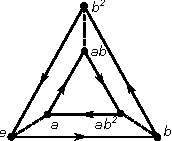
\includegraphics{img/chap5gdefn.pdf}}

    $\to$ means ``multiply by $b$''

    $\dashrightarrow$ means ``multiply by $a$''
    \end{center}

    \noindent Moving in the \emph{forward} direction of the arrow $\to$
    means multiplying by $b$,

    \begin{center} $x \to xb$ \end{center}

    \noindent whereas moving in the \emph{backward} direction of the
    arror means multiplying by $b^{-1}$:

    \begin{center} $x \leftarrow xb^{-1}$ \end{center}

    \noindent (Note that ``multiplying $x$ by $b$'' is understood to
    mean multiplying \emph{on the right} by $b$: it means $xb$, not
    $bx$.) It is also a convention that if $a^2=e$ (hence $a=a^{-1}$), then
    no arrowhead is used; for if $a=a^{-1}$, then multiplying by $a$
    is the same as multiplying by $a^{-1}$.

    The Cayley diagram of a group contains the same information as the group's
    table. For instance, to find the product $(ab)(ab^2)$ in the figure on
    page 51, we start as $ab$ and follow the path corresponding to $ab^2$
    (multiplying by $a$, then by $b$, then again by $b$) which
    is $\dashrightarrow \to\to$. This path leads to $b$; hence 
    $(ab)(ab^2)=b$.

    As another example, the inverse of $ab^2$ is the path which leads from
    $ab^2$ back to $e$. We not instantly that this is $ba$.

    Write the table of the groups having the following Cayley diagrams:
    (\textsc{Remark}: You may take any point to represent $e$, because
    there is perfect symmetry in a Cayley diagram. Choose $e$, then
    label the diagram and proceed.)
    

    \noindent 1. 
        \scalebox{.75}{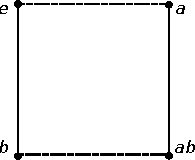
\includegraphics{img/chap5g1.pdf}}

    \noindent \solution The upper left corner
    was chosen as $e$. The $\dashrightarrow$ was associated with $a$. The
    $\to$ was associated with $b$. Since the lines actually don't show
    arrow heads we know that $a^2=b^2=e$. We also know it must
    be the case that we have the defining equation $ab=ba$.

    So the table is:
    \begin{center}
    \begin{tabular}{c|cccc}
       $\cdot$ & $e$ & $a$ & $b$ & $ab$ \\ \hline
       $e$     & $e$ & $a$ & $b$ & $ab$ \\
       $a$     & $a$ & $e$ & $ab$ & $b$ \\
       $b$     & $b$ & $ab$ & $e$ & $a$ \\
       $ab$    & $ab$ & $b$ & $a$ & $e$
    \end{tabular}
    \end{center}

    \noindent 2. \scalebox{1.0}{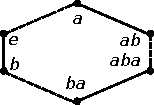
\includegraphics{img/chap5g2.pdf}}

    \noindent \solution Like 1, we chose $e$ to be upper left,
    $\dashrightarrow$ to represent $a$ and $\to$ to represent $b$.
    We have the defining equations $a^2=b^2=e$ and $bab=aba$. The
    group is $\{e,a,b,ab,ba,aba\}$.
    \begin{center}
    \begin{tabular}{c|cccccc}
    $\cdot$ & $e$ & $a$ & $b$ & $ab$ & $ba$ & $aba$ \\ \hline
    $e$     & $e$ & $a$ & $b$ & $ab$ & $ba$ & $aba$ \\ 
    $a$     & $a$ & $e$ & $ab$ & $b$ & $aba$ & $ba$ \\
    $b$     & $b$ & $ba$ & $e$ & $aba$ & $a$ & $ab$ \\
    $ab$    & $ab$ & $aba$ & $a$ & $ba$ & $e$ & $b$ \\
    $ba$    & $ba$ & $b$ & $aba$ & $e$ & $ab$ & $a$ \\
    $aba$   & $aba$ & $ab$ & $ba$ & $a$ & $b$ & $e$
    \end{tabular}
    \end{center}

    \noindent 3. 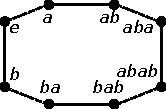
\includegraphics{img/chap5g3.pdf}

    \noindent \solution. Same conventions as 1 and 2 above. The group
    is $\{e,a,b,ab,ba,aba,bab,abab\}$. The defining equations are
    $a^2=b^2=e$, and $baba=abab$.
    \begin{center}
    \begin{tabular}{c|cccccccc}
    $\cdot$  & $e$ & $a$ & $b$ & $ab$ & $ba$ & $aba$ & $bab$ & $abab$\\\hline
    $e$      & $e$ & $a$ & $b$ & $ab$ & $ba$ & $aba$ & $bab$ & $abab$\\
    $a$      & $a$ & $e$ & $ab$ & $b$ & $aba$ & $ba$ & $abab$ & $bab$\\
    $b$      & $b$ & $ba$ & $e$ & $bab$ & $a$ & $abab$ & $ab$ & $aba$\\
    $ab$     & $ab$ & $aba$ & $a$ & $abab$ & $e$ & $bab$ & $b$ & $ba$\\
    $ba$     & $ba$ & $b$ & $bab$ & $e$ & $abab$ & $a$ & $aba$ & $ab$\\
    $aba$    & $aba$ & $ab$ & $abab$ & $a$ & $bab$ & $e$ & $ba$ & $b$\\
    $bab$    & $bab$ & $abab$ & $ba$ & $aba$ & $b$ & $ab$ & $e$ & $a$\\
    $abab$   & $abab$ & $bab$ & $aba$ & $ba$ & $ab$ & $b$ & $a$ & $e$
    \end{tabular}
    \end{center}

    \noindent 4. 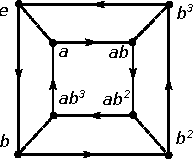
\includegraphics{img/chap5g4.pdf}

    \noindent \solution We can see this is the same group as 
    F2. This shape is probably where it gets its name. We copy the table
    from that exercise and you can visually check they are the same.

    \begin{center}
    \begin{tabular}{c|cccccccc}
    % -- heading row
    $\cdot$ & $e$ & $a$ & $b$ & $b^2$ & $b^3$ & $ab$ & $ab^2$ & $ab^3$ \\\hline

    % -- e row
    $e$ & $e$ & $a$ & $b$ & $b^2$ & $b^3$ & $ab$ & $ab^2$ & $ab^3$ \\

    % -- a row
    $a$ & $a$ & $e$ & $ab$ & $ab^2$ & $ab^3$ & $b$ & $b^2$ & $b^3$ \\

    % -- b row
    $b$ & $b$ & $ab^3$ & $b^2$ & $b^3$ & $e$ & $a$ & $ab$ & $ab^2$ \\

    % -- bb row
    % (bb)a = b(ba) = b(abbb) = (ba)bbb = (abbb)bbb = abb(bbbb) = abb
    $b^2$ & $b^2$ & $ab^2$ & $b^3$ & $e$ & $b$ & $ab^3$ & $a$ & $ab$ \\

    % -- bbb row
    % (bbb)a = bb(ba) = bb(abbb) = b(ba)bbb = b(abbb)bbb = (ba)bbbbbb
    %        = (abbb)bbbbbb = a(bbbb)(bbbb)b = ab
    $b^3$ & $b^3$ & $ab$ & $e$ & $b$ & $b^2$ & $ab^2$ & $ab^3$ & $a$ \\

    % -- ab row
    % (ab)a = a(ba) = a(abbb) = (aa)bbb = bbb
    $ab$ & $ab$ & $b^3$ & $ab^2$ & $ab^3$ & $a$ & $e$ & $b$ & $b^2$ \\

    % -- abb row
    % (abb)a = ab(ba) = ab(abbb) = a(ba)bbb = a(abbb)bbb = (aa)(bbbb)bb = bb
    $ab^2$ & $ab^2$ & $b^2$ & $ab^3$ & $a$ & $ab$ & $b^3$ & $e$ & $b$ \\

    % -- abbb row
    % (abbb)a = abb(ba) = abb(abbb) = ab(ba)(bbb) = ab(abbb)(bbb) 
    %         = a(ba)(bbb)(bbb) = a(abbb)(bbb)(bbb) = (aa)(bbbb)(bbbb)b = b    
    $ab^3$ & $ab^3$ & $b$ & $a$ & $ab$ & $ab^2$ & $b^2$ & $b^3$ & $e$
    \end{tabular}
    \end{center}

    \noindent 5. 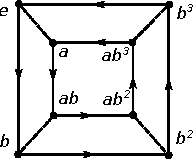
\includegraphics{img/chap5g5.pdf}

    \noindent \solution This is similar to last one, but the 
    defining equations are $a^2=e$, $b^4=e$, and $ba=ab$. The 
    group is $\{e,a,b,b^2,b^3,ab^2,ab^3\}$. The table is

    \begin{center}
    \begin{tabular}{c|cccccccc}
    $\cdot$  & $e$ & $a$ & $b$ & $b^2$ & $b^3$ & $ab$ & $ab^2$ & $ab^3$\\\hline
    $e$      & $e$ & $a$ & $b$ & $b^2$ & $b^3$ & $ab$ & $ab^2$ & $ab^3$\\
    $a$      & $a$ & $e$ & $ab$ & $ab^2$ & $ab^3$ & $b$ & $b^2$ & $b^3$\\
    $b$      & $b$ & $ab$ & $b^2$ & $b^3$ & $e$ & $ab^2$ & $ab^3$ & $a$\\
    $b^2$    & $b^2$ & $ab^2$ & $b^3$ & $e$ & $b$ & $ab^3$ & $a$ & $ab$\\
    $b^3$    & $b^3$ & $ab^3$ & $e$ & $b$ & $b^2$ & $a$ & $ab$ & $ab^2$\\
    $ab$     & $ab$ & $b$ & $ab^2$ & $ab^3$ & $a$ & $b^2$ & $b^3$ & $e$\\
    $ab^2$   & $ab^2$ & $b^2$ & $ab^3$ & $a$ & $ab$ & $b^3$ & $e$ & $b$\\
    $ab^3$   & $ab^3$ & $b^3$ & $a$ & $ab$ & $ab^2$ & $e$ & $b$ & $b^2$
    \end{tabular}
    \end{center}

    \noindent 6. 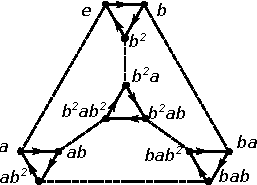
\includegraphics{img/chap5g6.pdf}

    \noindent \solution The equations are $baba = ab^2$, $a^2=e$, and $b^3=e$. 
    The group is $\{e,a,ab,ab^2,b,b^2,ba,bab,bab^2,b^2a,b^2ab,b^2ab^2\}$ 
    See the result in table~\ref{tab:g6}.
\begin{table}
\caption{The table for exercise G6.}
\label{tab:g6}
\begin{tabular}{c|cccccccccccc}
$\cdot$ & $e$ & $a$ & $ab$ & $ab^2$ & $b$ & $b^2$ & $ba$ & $bab$ & $bab^2$ &
   $b^2a$ & $b^2ab$ & $b^2ab^2$ \\\hline

$e$ & $e$ & $a$ & $ab$ & $ab^2$ & $b$ & $b^2$ & $ba$ & $bab$ & $bab^2$ &
   $b^2a$ & $b^2ab$ & $b^2ab^2$ \\

%a(ba) = (e)aba = (bbb)aba = bb(baba) = bb(abb) 
%a(bba) = (abb)a = (baba)a = (bab)(aa) = bab
$a$ & $a$ & $e$ & $b$ & $b^2$ & $ab$ & $ab^2$ & $b^2ab^2$ & $b^2a$ & $b^2ab$ &
    $bab$ & $bab^2$ & $ba$\\

%ab(ba) = (abb)a = (baba)a = (bab)(aa) = bab
$ab$ & $ab$ & $b^2ab^2$ & $b^2a$ & $b^2ab$ & $ab^2$ & $a$ & $bab$ & $bab^2$ &
   $ba$ & $e$ & $b$ & $b^2$\\ 

%abb(a) = (baba)a = (bab)(aa) = (bab)
$ab^2$ & $ab^2$ & $bab$ & $bab^2$ & $ba$ & $a$ & $ab$ & $e$ & $b$ & $b^2$ &
  $b^2ab^2$ & $b^2a$ & $b^2ab$   \\

$b$ & $b$ \\

$b^2$\\
$ba$\\
$bab$\\
$bab^2$\\
$b^2a$\\
$b^2ab$\\
$b^2ab^2$\\
\end{tabular}
\end{table}

\begin{verbatim}

\end{verbatim}
   \noindent Just for fun I wanted to do a Cayley Diagram of the 
   group $\langle \mathbb{Z}_{10}, + \rangle$ which we learned
   in E2 can be generted by 2 and 5. See figure~\ref{fig:cayleyZ10}.

   \begin{figure}
   \caption{A Cayley Diagram of $\langle\mathbb{Z}_{10}, + \rangle$.}
   \label{fig:cayleyZ10}
   \vspace{10pt}
   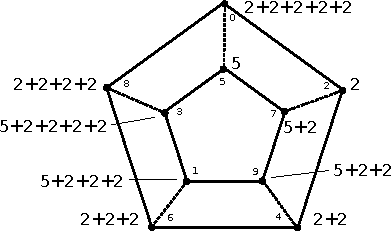
\includegraphics{img/modulo10Cayley.pdf}
   \end{figure}

   \vspace{10pt}
   \item\textsc{Coding Theory: Generator Matrix and Parity-Check Matrix
   of a Code}

   \noindent 1. Find the generator matrix $\mathbf{G}_2$ and the
   parity-check matrix $\mathbf{H}_2$ of the code $C_2$ described
   in Exercise G2 of Chapter 3.

   \noindent \solution The generator matrix is
   \begin{align*}
       \mathbf{G}_2 & = \begin{pmatrix}
                          1 & 0 & 0 & 0 & 1 & 1 \\
			  0 & 1 & 0 & 1 & 1 & 1 \\
			  0 & 0 & 1 & 0 & 0 & 1
                        \end{pmatrix}
   \end{align*}

   \noindent The parity-check matrix can be calculated once
   we rewrite the parity-check equations: $a_4=a_2$, $a_5=a_1+a_2$,
   and $a_6=a_1+a_2+a_3$. They are $a_2+a_4=0$, $a_1+a_2+a_5=0$,
   and $a_1+a_2+a_3+a_6=0$.

   \begin{align*}
       (a_1,a_2,a_3,a_4,a_5,a_6)\cdot(0,1,0,1,0,0) &= 0 \\
       (a_1,a_2,a_3,a_4,a_5,a_6)\cdot(1,1,0,0,1,0) &= 0 \\
       (a_1,a_2,a_3,a_4,a_5,a_6)\cdot(1,1,1,0,0,1) &= 0
   \end{align*}

   Therefore,
   \begin{align*}
       \mathbf{H}_2 & =
          \begin{pmatrix}
	    0 & 1 & 0 & 1 & 0 & 0 \\
	    1 & 1 & 0 & 0 & 1 & 0 \\
	    1 & 1 & 1 & 0 & 0 & 1
	  \end{pmatrix}
   \end{align*}

   \noindent 2. Let $C_3$, be the following code in $\mathbb{B}^7$: the first
   four positions are information positions, and the parity-check equations
   are $a_5=a_2+a_3+a_4$, $a_6=a_1+a_3+a_4$, and $a_7=a_1+a_2+a_4$.
   ($C_3$ is called the \emph{Hamming code}.) Find the generator matrix
   $\mathbf{G}_3$ and the parity-check matrix $\mathbf{H}_3$ of $C_3$.

   \noindent \solution The generator matrix is:
   \begin{align*}
      \mathbf{G}_3 & = 
         \begin{pmatrix}
	    1 & 0 & 0 & 0 & 0 & 1 & 1 \\
	    0 & 1 & 0 & 0 & 1 & 0 & 1 \\
	    0 & 0 & 1 & 0 & 1 & 1 & 0 \\
	    0 & 0 & 0 & 1 & 1 & 1 & 1
	 \end{pmatrix}
   \end{align*}

   The parity-check equations can be rewritten: $a_2+a_3+a_4+a_5=0$,
   $a_1+a_3+a_4+a_6=0$, and $a_1+a_2+a_4+a_7=0$. 

   \begin{align*}
       (a_1,a_2,a_3,a_4,a_5,a_6,a_7)\cdot(0,1,1,1,1,0,0) &= 0\\
       (a_1,a_2,a_3,a_4,a_5,a_6,a_7)\cdot(1,0,1,1,0,1,0) &= 0\\
       (a_1,a_2,a_3,a_4,a_5,a_6,a_7)\cdot(1,1,0,1,0,0,1) &= 0
   \end{align*}
   
   Therefore,
   \begin{align*}
      \mathbf{H}_3 &= 
         \begin{pmatrix}
	    0 & 1 & 1 & 1 & 1 & 0 & 0 \\
	    1 & 0 & 1 & 1 & 0 & 1 & 0 \\
	    1 & 1 & 0 & 1 & 0 & 0 & 1
	 \end{pmatrix}
   \end{align*}

   \vspace{10pt}
   The \emph{weight} of a word $\mathbf{x}$ is the number of 1s in the
   word and is denoted by $w(\mathbf{x})$. For example,
   $w(11011)=4$. The \emph{minimum weight} of a code $C$ is the weight
   of the nonzero codeword of smallest weight in the code.
   Prove the following:

   \noindent 3 $d(\mathbf{x},\mathbf{y})=w(\mathbf{x}+\mathbf{y})$.

   \noindent \begin{proof}
   The distance between $\mathbf{x}$ and $\mathbf{y}$ is the number of
   positions in which they differ. Let $\mathbf{x}_i$ and $\mathbf{y}_i$
   be the values of $\mathbf{x}$ and $\mathbf{y}$, respctively,
   at position $i$.
   If they differ then $\mathbf{x}_i + \mathbf{y}_i=1$. If they
   are equal then $\mathbf{x}_i + \mathbf{y}_i = 0$. So at every 
   position where the two words differ we get a 1 for their sum,
   and for every position where they are the same we get a 0 for their
   sum. Therefore, when we add both words together we get a 1
   in precisely every location where the two values differ and therefore
   $d(\mathbf{x},\mathbf{y})=w(\mathbf{x}+\mathbf{y})$.

   More precisely we define the function 

   \[
      d(\mathbf{x},\mathbf{y}) = \sum_{i=1}^{n}d'(\mathbf{x}_i,\mathbf{y}_i) \tag{Difference}
   \]
   where we define the function $d'$ to generate a 1 if two bits
   are different and 0 if two bits are equal.
   \[
      d'(\mathbf{x}_i,\mathbf{y}_i) = 
	 \begin{cases}
	    0,   &\text{if $\mathbf{x}_i = \mathbf{y}_i$;}\\
	    1,   &\text{otherwise.}
	 \end{cases}
   \]
   Next we show that $w(\mathbf{x}+\mathbf{y})$ is
   $w(\mathbf{x}_n\ldots\mathbf{x}_1 + \mathbf{y}_n\ldots\mathbf{y}_1)$.
   This can be rewritten as $w((\mathbf{x}_n+\mathbf{y}_n)\ldots
   (\mathbf{x}_1+\mathbf{y}_1))$ or

   \[
      w(\mathbf{x}+\mathbf{y}) = \sum_{i=1}^{n} \mathbf{x}_i+\mathbf{y}_i 
         \tag{Weight}
   \]

   Now notice that the two summations in the equations labelled
   Difference and Weight are exactly identical. This is because
   the addition of bits used in (Weight) is identical to the difference
   of bits used in (Difference).
   \end{proof}

   \noindent 4. $w(\mathbf{x})=d(\mathbf{x},\mathbf{0})$, where
   $\mathbf{0}$ is the word whose digits are all 0s.

   \noindent 
   \begin{proof}This follows immediately from H3 since
   $\mathbf{x}=\mathbf{x}+\mathbf{0}$. Therefore, $w(\mathbf{x})=
   w(\mathbf{x}+\mathbf{0})$ and therefore by H3 this is equal
   to $d(\mathbf{x},\mathbf{0})$.
   \end{proof}

   \noindent 5. The minimum distance of a group code $C$ is equal
   to the minimum weight of $C$. 

   \begin{proof}
   There must be a neutral element since this is a group. This
   neutral element is $\mathbf{0}$. The hypothesis suggests that
   there is no element \emph{closer} in distance to a minimum
   weight word than the word $\mathbf{0}$. In this proof,
   I will assume there is and prove a contradiction, thereby
   proving the hypothesis.

   Suppose $\mathbf{x}$ is a word with minimum weight in $C$, and
   assume their exists another word $\mathbf{y}$ in $C$
   such that $d(\mathbf{x},\mathbf{y}) <
   d(\mathbf{x},\mathbf{0})$.  Let's consider the word
   $\mathbf{x}+\mathbf{y}$ which we know exists in $C$ since it is a group.
   We know from H3 that 
   $d(\mathbf{x},\mathbf{y})=w(\mathbf{x}+\mathbf{y})$. 
   Therefore $w(\mathbf{x}+\mathbf{y}) < d(\mathbf{x},\mathbf{0}) =
   w(\mathbf{x})$. So $\mathbf{x}+\mathbf{y}$ is of lesser weight
   then $\mathbf{x}$. But this contradicts the fact that $\mathbf{x}$
   is of minimum weight. Therefore no such word $\mathbf{y}$ exists.
   \end{proof}



\end{enumerate}


\end{document}
